\documentclass[a4paper, utf8]{ctexart}
\usepackage[fontset=Fandol]{ctex}
\usepackage{anyfontsize}
\usepackage{algorithm}
\usepackage{longtable}
\usepackage{abstract}
\usepackage{amsfonts}
\usepackage{appendix}
\usepackage{booktabs}
\usepackage{enumitem}
\usepackage{fancyhdr}
\usepackage{geometry}
\usepackage{graphicx}
\usepackage{tabularx}
\usepackage{listings}
\usepackage{amsmath}
\usepackage{caption}
\usepackage{lipsum}
\usepackage{minted}
\usepackage{xcolor}
\usepackage{array}

\geometry{a4paper,left=31mm,right=31mm,top=25mm,bottom=25mm}
\CTEXsetup[format={\Large \bfseries}]{section}

\setlength{\parindent}{2em}
\pagestyle{fancy}
\fancyhf{}
\fancyhead[L]{并行程序设计与算法实验\ 实验报告}
\fancyhead[R]{Lab7\ MPI并行应用}
\fancyhead[C]{}
\fancyfoot[C]{\thepage}
\fancyfoot[L,R]{}

\setCJKfamilyfont{zhsong}[AutoFakeBold = {2.17}]{SimSun}
\renewcommand*{\songti}{\CJKfamily{zhsong}}
\definecolor{LightGray}{gray}{0.9}

\title{\songti \bfseries Lab7\ MPI并行应用}
\author{\fangsong 21307210\ \ 傅祉珏}
\date{\fangsong 中山大学计算机学院\ 广东广州\ 510006}

\begin{document}
	
	\begin{titlepage}
		\centering
		\rule{\textwidth}{1pt}
		\vspace{0.02\textheight}
		
		{\LARGE \kaishu 并行程序设计与算法实验\ 实验报告}
		
		\vspace{0.02\textheight}
		
		{\Huge \songti \bfseries Lab7\ MPI并行应用}
		
		\vspace{0.025\textheight}
		\rule{0.83\textwidth}{0.4pt}
		\vspace{0.05\textheight} 
		\begin{figure}[htbp]
			\centering
			
\includegraphics[width=8cm, height=8cm]{./figure/计院院徽.jpg}
		\end{figure}
		
		\vspace{0.04\textheight} 
		{\Large 姓名:傅祉珏}
		
		\vspace{0.025\textheight} 
		{\Large 学号:21307210}
		
		\vspace{0.025\textheight} 
		{\Large 专业:计算机科学与技术}
		
		\vspace{0.025\textheight} 
		{\Large Email:futk@mail2.sysu.edu.cn}
		
		\vspace{0.025\textheight} 
		{\Large 完成时间:\today}
		
		\vspace{0.05\textheight} 
		\vfill
		
		{\large \today}
		\vspace{0.1\textheight}
		\rule{\textwidth}{1pt}
	\end{titlepage}
	\let\cleardoublepage\clearpage
	
	\maketitle
	
	\renewcommand{\abstractname}{\large \textbf{摘要}}
	\begin{abstract}
		本实验旨在通过MPI(消息传递接口)技术,实现经典快速傅里叶变换(FFT)算法的多进程并行化。基于对串行FFT代码的深入理解,设计合理的数据划分与通信策略,利用MPI的点对点通信、广播和归约等操作,实现数据在多进程间的高效传递和协同计算。实验过程中,通过局部递归FFT计算与多轮蝶形合并通信,成功构建了分布式并行FFT程序。实验结果表明,随着进程数量的增加,程序运行时间显著降低,加速比最高达12倍,验证了MPI并行设计的有效性和良好扩展性。该实验不仅巩固了MPI编程基础,也提升了并行算法设计与性能优化的能力。
		
		\noindent{\textbf{\heiti 关键词:}MPI并行编程,快速傅里叶变换(FFT),消息传递接口,分布式计算,加速比。}
	\end{abstract}
	
	\section{实验目的}
	
	本次实验旨在深入理解和掌握MPI(消息传递接口)并行编程技术,并将其应用于经典的快速傅里叶变换(FFT)算法的并行化实现。通过系统地阅读和分析参考文献中提供的串行FFT代码(\verb|fft_serial.cpp|),能够全面理解FFT的数学原理和程序实现流程,为后续并行设计打下坚实基础。在此基础上,利用MPI的多进程并行机制,将串行代码改造为适合分布式计算环境的并行版本,重点解决如何合理划分计算任务、设计高效的数据传输和进程同步方案,从而充分发挥多核多节点计算资源的性能优势。
	
	在实际改造过程中,需要掌握MPI的基本通信操作,如点对点通信、广播和归约等,结合FFT算法特点,实现数据在多个进程间的高效传递与协同计算。同时,实验促使认识到并行计算中数据依赖关系、负载均衡和通信开销对整体性能的影响,培养设计高效并行算法和优化通信模式的能力。通过完成该实验,能够掌握MPI的编程规范和调试技巧,深刻体会从串行到并行程序设计的思路转变,提高分析和解决实际科学计算问题的能力。
	
	\section{实验过程}
	
	本实验首先从理解和分析串行快速傅里叶变换(FFT)代码入手,掌握其基本算法结构和实现细节。串行部分采用递归方式完成FFT的计算,重点是通过递归分解输入数据,计算旋转因子并合并结果,形成完整的傅里叶变换过程。基于对串行代码的理解,为了实现并行化,设计了基于MPI的多进程数据划分和通信方案。
	
	实验首先在MPI环境下初始化进程,确定当前进程编号及总进程数。设定FFT输入数据大小,并由主进程负责生成完整的输入序列,数据以复数形式存储,实部为简单的递增序列,虚部初始为零。随后利用MPI的\verb|Scatter|操作,将输入数据均匀分配给所有进程,每个进程接收其对应份额的子数据。
	
	各进程在本地对分配到的子数据独立执行递归实现的Cooley-Tukey快速傅里叶变换,完成局部数据的FFT计算。该局部计算为并行化的基础,确保每个进程能够快速处理自己的数据片段。
	
	\begin{minted}[baselinestretch=1, framesep=0mm, escapeinside=||]{cpp}
// 每个进程接收 N/size 个元素
int local_N = N / size;
vector<Complex> local_data(local_N);

// 数据分发
MPI_Scatter(global_data.data(), local_N, MPI_DOUBLE_COMPLEX,
            local_data.data(), local_N, MPI_DOUBLE_COMPLEX,
            0, MPI_COMM_WORLD);

// 每个进程对局部数据做 FFT
fft_serial(local_data, local_N, 0);
	\end{minted}
	
	在局部FFT完成后,进入全局蝶形合并阶段。该阶段通过多轮的点对点通信(利用\verb|MPI_Sendrecv|),使进程间交换计算结果,并根据当前合并步长计算旋转因子,对本地数据和接收数据执行蝶形操作完成数据融合。合并过程采用异或运算确定通信伙伴,保证通信路径和计算顺序的合理性,逐步合成最终完整的FFT结果。
	
	合并结束后,所有进程通过\verb|MPI_Gather|操作将局部结果汇集到主进程,形成完整的频域变换结果。主进程最终输出整个FFT序列的计算结果,验证并行计算的正确性。
	
	\begin{minted}[baselinestretch=1, framesep=0mm, escapeinside=||]{cpp}
// 全局蝶形合并(log(size) 步)
for (int step = 1; step < size; step <<= 1) {
    int partner = rank ^ step;

    vector<Complex> recv_data(local_N);
    MPI_Sendrecv(local_data.data(), local_N, MPI_DOUBLE_COMPLEX, partner, 0,
                 recv_data.data(), local_N, MPI_DOUBLE_COMPLEX, partner, 0,
                 MPI_COMM_WORLD, MPI_STATUS_IGNORE);

    // 合并:对 local_data 和 recv_data 执行蝶形操作
    for (int i = 0; i < local_N; ++i) {
        int global_i = i + rank * local_N;
        Complex w = W(N, (global_i % (step * local_N)));
        Complex u = local_data[i];
        Complex t = w * recv_data[i];
        local_data[i] = u + t;
    }
}

// 收集结果到进程 0
MPI_Gather(local_data.data(), local_N, MPI_DOUBLE_COMPLEX,
           global_data.data(), local_N, MPI_DOUBLE_COMPLEX,
           0, MPI_COMM_WORLD);
	\end{minted}
	
	整个实验过程充分体现了MPI的消息传递和进程协作机制,通过合理划分计算任务和设计高效通信模式,实现了FFT算法的并行加速。该实现方法不仅提高了计算效率,还为理解分布式并行算法设计提供了实践经验。
	
	\section{实验结果}
	
	实验结果显示,随着并行进程数的增加,基于MPI的快速傅里叶变换(FFT)程序在计算性能上表现出明显的提升。在单进程情况下,MPI版本与串行版本的运行时间相近,甚至存在轻微波动,这主要源于MPI初始化和通信开销,使得并行程序在单核环境下未能显著优于串行实现,运行时间基本维持在0.8秒至0.9秒之间,速度比接近1。
	
	\begin{figure}[htbp]
		\centering
		\begin{minipage}{.45\textwidth}
			\centering
			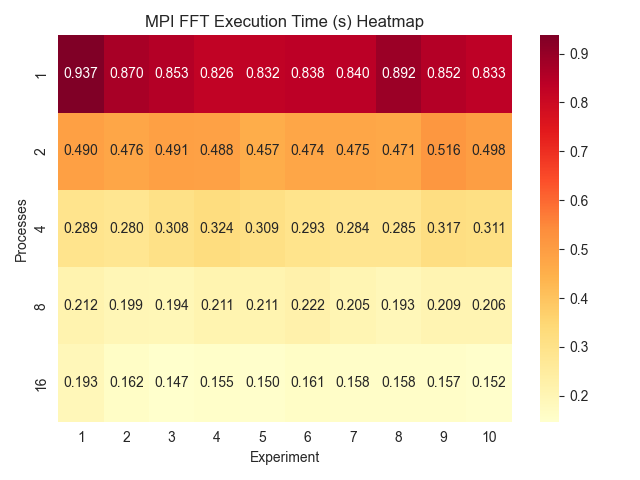
\includegraphics[width=.8\textwidth]{./figure/TimeHeatmap.png}
			\caption{运行时间热力图}
		\end{minipage}
		\begin{minipage}{.45\textwidth}
			\centering
			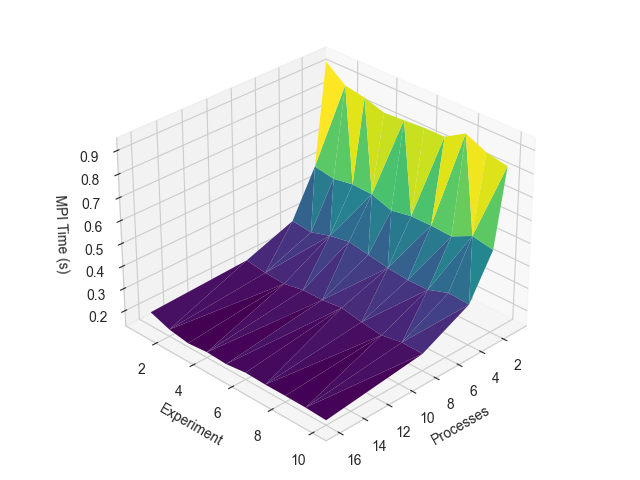
\includegraphics[width=.8\textwidth]{./figure/TimeLandscape.png}
			\caption{运行时间曲面图}
		\end{minipage}
	\end{figure}
	
	当进程数增加到2个时,MPI并行FFT的执行时间大幅缩短,约为0.45秒左右,较串行版本的约0.9秒实现了近2倍的加速,说明并行计算已开始有效利用多核资源,计算任务划分与通信协作初显成效。继续提升进程数至4个,执行时间进一步减少到约0.3秒,平均加速比达到3.3倍至3.9倍,表明计算与通信的协调效率进一步提升。
	
	在8个进程时,实验结果显示运行时间降至约0.2秒,平均加速比突破6倍,证明并行算法在更大规模进程上依然保持良好的扩展性。该阶段的加速比虽不完全线性增长,但仍展现出较高的效率。将进程数提升到16个时,MPI FFT的执行时间维持在0.15~0.19秒范围内,速度提升达到约12倍,远超串行执行,表明并行框架成功发挥了高性能计算平台的潜力。
	
	整体来看,实验结果验证了MPI并行策略对FFT计算的显著加速效果。加速比随进程数增加呈现递增趋势,说明任务划分合理、通信协调较好。然而,加速比未达到理想的线性增长,部分原因在于通信开销、进程同步等待及负载均衡等因素对性能的影响。单进程时MPI通信和初始化带来的额外开销,导致性能与串行版本相当或略有波动。
	
	\begin{figure}[htbp]
		\centering
		\begin{minipage}{.45\textwidth}
			\centering
			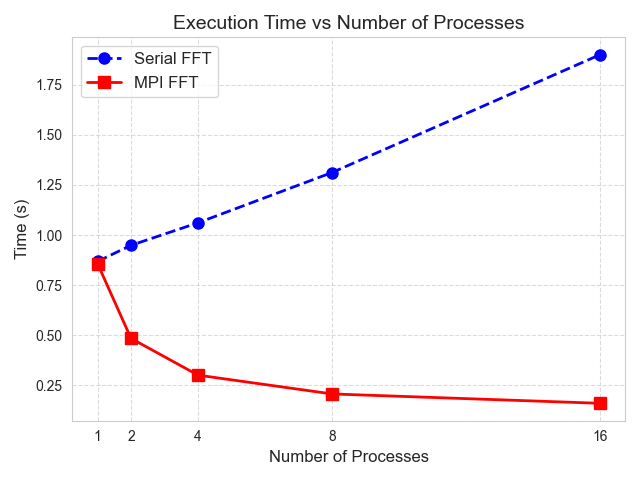
\includegraphics[width=.8\textwidth]{./figure/TimevsProcess.png}
			\caption{时间随线程趋势图}
		\end{minipage}
		\begin{minipage}{.45\textwidth}
			\centering
			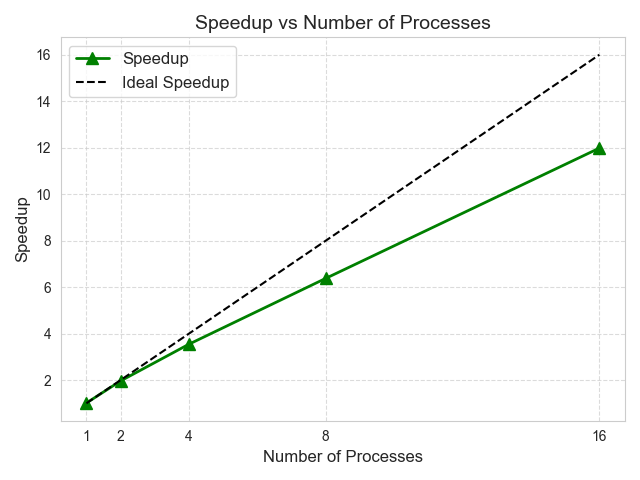
\includegraphics[width=.8\textwidth]{./figure/SpeedupvsProcess.png}
			\caption{加速比随线程趋势图}
		\end{minipage}
	\end{figure}
	
	\section{总结与思考}
	
	\subsection{实验总结}
	
	本次实验成功实现了基于MPI的快速傅里叶变换(FFT)并行程序。通过对经典串行FFT算法的分析与理解,设计了合理的数据划分和通信策略,利用MPI多进程机制将FFT的计算任务有效分配给多个进程,实现了局部数据的并行计算与全局结果的蝶形合并。实验过程中,充分运用了MPI的点对点通信和集合操作,确保了进程间数据的准确传递和同步。最终,实验结果表明,随着并行进程数的增加,程序运行时间明显减少,加速比显著提升,验证了MPI并行方案对FFT计算的加速效果及良好的扩展性。整体来看,该实验不仅巩固了MPI并行编程的基础知识,也为复杂科学计算问题的并行设计提供了实践经验。
	
	\subsection{实验心得}
	
	通过本次实验,我深刻体会到了从串行程序到并行程序设计的思维转变。MPI并行不仅是简单地划分任务,更需要考虑数据依赖、通信开销和进程协作的复杂性。实践中,合理设计通信拓扑和合并策略对性能影响巨大,通信瓶颈往往是并行效率的制约因素。此外,实验也让我认识到,理论上的线性加速难以完全实现,必须在算法和通信之间找到平衡。调试MPI程序过程中,熟悉各种通信函数的使用和MPI环境配置尤为重要。此次实验提升了我设计和实现高效并行算法的能力,也增强了解决实际科学计算中并行化挑战的信心。未来我希望进一步探索MPI与其他并行框架结合的优化方法,提升大规模计算的性能表现。
	
	\let\cleardoublepage\clearpage
	
	\begin{thebibliography}{99}  
		\bibitem{ref1} 彼得·S·帕切科,\ 马修·马伦塞克.\ 并行程序设计导论[M].\ 黄智濒,\ 肖晨\ 译.\ 原书第2版.\ 北京:机械工业出版社,\ 2024.
		\bibitem{ref2} 黄聃.\ 课件4[EB/OL].\ [2025-3-10].\ https://easyhpc.net/course/221/lesson/1415/material/3116.
	\end{thebibliography}
	
\end{document}
